%%%%%%%%%%%%%%%%%%%%%%%%%%%%%%%%%%%%%%%%%%%%%%%%%%%%%%%%%%%%%%%%%%%%%%%%%%%%%%%%
% Section 1
\section{Genome Assembly Problem}

\begin{frame}
\frametitle{DNA Assembly}
Within the last two decades, \textbf{assembling a genome from an enormous amount of reads} from various DNA sequencers has been one of the most challenging computational problems in molecular biology.
\\ \medskip
Such a problem is proved to be NP-hard and many algorithms have been devised to come to a solution both exact and approximated.
\\ \medskip
There are two types of algorithms that are commonly utilized by assemblers:
\begin{itemize}
\item \textbf{Greedy}, which aim for local optima,
\item \textbf{Graph methods}, which aim for global optima.
\end{itemize}
\end{frame}

\begin{frame}
\frametitle{Graph methods (Waterman and Gene Myers 1994)}
Graph-method-assemblers come in two varieties: the ones based on \textbf{overlap graph} and the others based on \textbf{de Bruijn graphs}.
\\ \medskip 
These methods represented an important step forward in sequence assembly, as they both use algorithms to reach a global optimum instead of a local one.
Thanks to these theoretical advances computational genomics over large volumes of data became an easier problem to attack.
\\ \medskip
Both of these methods made progress towards better assemblies  but nowadays the De Bruijn graph method has become the most popular due to the so called \textcolor{red}{next-generation sequencing machines}.
\end{frame}

\begin{frame}
\frametitle{The Overlap graph}
Most assembly algorithms from the \textit{"Sanger era"}
are based on the \textbf{overlap graph}.
\\ \medskip
Such a graph has one node for each read produced by the sequencing process and two nodes are connected by a weighted edge iff the corresponding two reads have an overlap of enough length. \textit{(this length is a parameter of the implementation)}
\begin{figure}
	Read set $\mathcal{R} = \{CTCTAGGCC, GCCCTCAAT, CAATTTTT\}$
	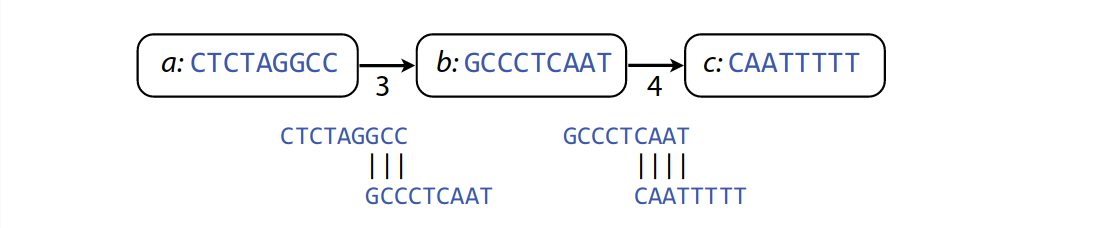
\includegraphics[scale=0.33]{img/overlap-graph-simple.png}
\end{figure}
\end{frame}


\begin{frame}
\frametitle{Shortest common superstring and TSP}
\begin{columns}
	\column{0.5\textwidth}
	By adding a minus sign in front of each edge label we get into a framework
	such that the assembly problem is reduced to the \textbf{Shortest common superstring problem} that indeed is equivalent to \textbf{TSP}, one of the most famous NP-HARD problems.
	\column{0.5\textwidth}
	\begin{figure}
		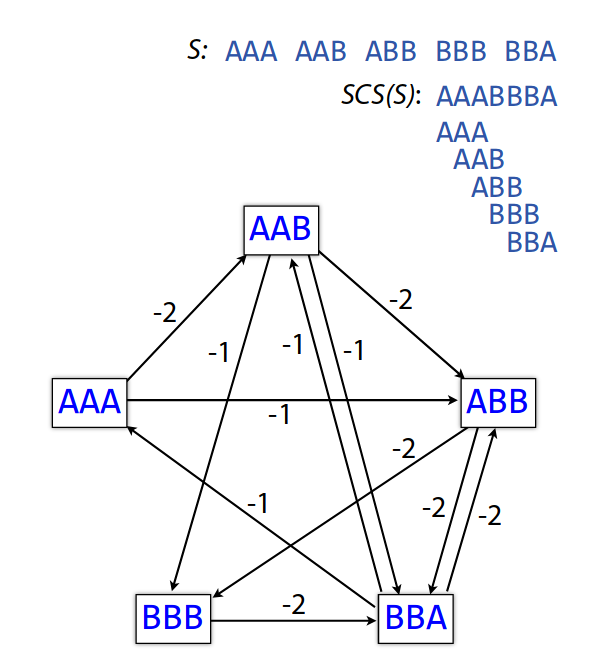
\includegraphics[scale=0.25]{img/tsp-scs.png}
	\end{figure}
\end{columns}
\end{frame}

\begin{frame}
\frametitle{New Generation Sequencing}
This strategy is too expensive to apply against the huge data from most recent \textbf{next-generation sequencers } (NGSs). 
\\ \medskip
NGS machines can sequence vast amount of genome data. 
\\
It makes it computationally not tractable to compare all the pairs of reads to find the optimal solution for \textbf{SCS}. 
\\ \medskip
Moreover, most NGSs cannot read long DNA fragments (e.g., at most 200bp in the case of Illumina HiSeq2000),
and their read lengths are not long enough to detect overlaps with enough lengths between reads.
\end{frame}

\begin{frame}
\frametitle{New Generation Sequencing - Shotgun sequencing}
\begin{columns}
	\column{0.45\textwidth}
	One current popular NGS method is \textbf{shotgun sequencing}, which:
	\begin{itemize}
		\item  clones the genome a bunch of times,
		\item  then randomly breaks each clone into short segments
	\end{itemize}
	the fact that we randomly cut many clones of the same DNA segment should lead to have overlapping reads.
	\column{0.55\textwidth}
	\begin{figure}
		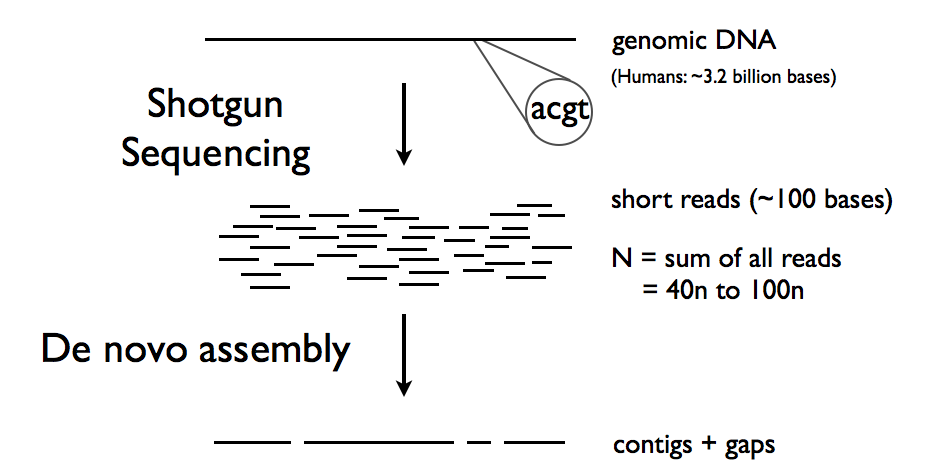
\includegraphics[scale=0.2]{img/shotgun.png}
	\end{figure}
\end{columns}
\end{frame}

\begin{frame}
\frametitle{de Bruijn graph}
\begin{columns}
	\column{0.6\textwidth}
To conquer these problems, many recent assembler algorithms utilize a
graph called the de Bruijn graph.
\\ \medskip
This kind of graphs is really suitable to represent a large network of overlapping \textbf{short read data}.
\\ \medskip
In this model each node represents a \textbf{k-mer} that exists in the reads, and an edge exists iff there is an exact
overlap of length \textbf{k−1} between the corresponding k-mers.
	\column{0.4\textwidth}
	\begin{figure}
	Example read $R =TACGACGTCGACT$
	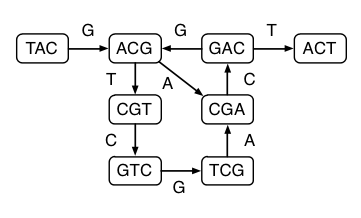
\includegraphics[scale=0.4]{img/dbg-graph-simple.png}
	\end{figure}
\end{columns}
\end{frame}

%\begin{frame}
%\frametitle{de Bruijn graph in Bioinformatics}
%During the assembly of the De Bruijn graph, reads are broken into smaller fragments of a specified size, k.
%\\ \medskip
%The k-mers are then used as nodes in the graph assembly.\\
%Nodes that overlap by some amount (generally, k-1) are connected by a labelled edge.
%\\ \medskip
%The assembler will construct sequences based on the De Bruijn graph. 
%\end{frame}

\begin{frame}
\frametitle{Eulerian path in de Bruijn graphs}
After having built such a graph our original problem reduced to find \textbf{Eulerian paths} in it
\\ \medskip
Assuming \textbf{perfect sequencing} where each length-k substring is sequenced exactly once with no errors,\\
the naive "sliding-window" procedure to build the dBG always yields an Eulerian graph.
\end{frame}

\begin{frame}
\frametitle{dBG PRO and CONS}
The Single most important benefit of De Bruijn graph assemblers is speed and simplicity.
\\ \medskip
But since reads are immediately split into shorter k-mers
\begin{itemize}
	\item Information about contexts longer than k is lost
	\item Read coherence is lost: some paths through De Bruijn graph are inconsistent with respect to input reads. \\
	\item dBGs need to be preprocessed because of an high probability of sequening errors (tips, bubbles ...)
\end{itemize}
\end{frame}

\begin{frame}
\frametitle{Real world cases need something smaller and faster!}
de Bruijn graphs can be constructed more efficiently than the overlap graph in many cases, but naive procedures still remain a bottleneck in term of used space.
\\ \medskip
This is because storing all the edges of the de Bruijn graph requires huge amount of memory.
\\ \medskip 
Thus the focus of this presentation is on reducing the memory required for the de Bruijn graphs deploying some smart compression technique.
\end{frame}